\begin{frame}{Evaluation Criteria}
  \small{\begin{itemize}
  \item \textbf{Efficiency}\\
    %\begin{definition}
    Call a robot $r_i$ \textbf{static} at time $t$ if its pose $p_i$
    remains the same at all future times.
   % $$p_i(t') = p_i(t) \quad \mbox {for all } t' > t$$    
  %\end{definition}
    Define the \textbf{execution time} $\bar{t}$ of the system as the
    smallest time when all the robots reach static positions
  \item \textbf{Quality} \\
    When all robots reach static positions, for a robot $r_i$ with
    $N_i$ neighbors and $E_i$ outgoing edges, define a non-fulfillment
    ratio $\Gamma$ to measure the overall lattice quality
    $$\Gamma = \dfrac{1}{n}\sum\limits_{i=1}^n \frac{E_i - N_i}{E_i}$$
  \end{itemize}
  }
  \begin{columns}[T] 
    \begin{column}{.4\textwidth}
        \begin{figure}
  \centering
  \begin{tikzpicture}[distance=1cm]
    %->,>=stealth',shorten >=5pt,auto,node          ]
    \tikzstyle{every state}=[fill=myred, draw=none, text=white]
    \node[state, scale=0.5] (A) at (0,0)    {$0$};
    \node[state, scale=0.5, fill=mycyan] (B) at (3,0)  {$1$};
    \path (A) edge [bend left=10] node {\scriptsize{Tr(0, 40)}} (B)
    (A) edge [bend left=45] node {\scriptsize{Tr(-35,-20)}} (B)
    (A) edge [bend left=90] node {\scriptsize{Tr(35,-20)}} (B)
    (B) edge [bend left=10] node {\scriptsize{Tr(-40,0)}} (A)
    (B) edge [bend left=45] node {\scriptsize{Tr(35,20)}} (A)
    (B) edge [bend left=90] node {\scriptsize{Tr(-35,20)}} (A);
  \end{tikzpicture}
\end{figure}
    \end{column}%
    \begin{column}{.5\textwidth}
      \begin{figure}
        \centering
        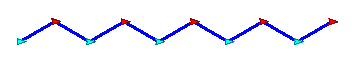
\includegraphics[width=0.6\linewidth]{figs/bad-hexagon}
      \end{figure}
      \begin{figure}
        \centering
        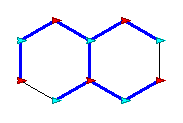
\includegraphics[scale=0.65]{figs/good-hexagon}
      \end{figure}
    \end{column}%
  \end{columns}
\end{frame}